\chapter{Interoperability: Managed Code vs. Native Code}
\label{chap:managed-code_native-code}

This chapter discusses how to interoperate managed code (written in any .NET languages)
with native code (written in C/C++). 

\section{Managed vs. Native code}

\subsection{Managed Code}
\label{sec:managed_code}

Code written using a .NET languages (C\#, J\#, VB.NET, JScript.NET) are called
{\bf managed code}. Managed code is the concept introduced since .NET Framework
1.0 and C\# 1.0.
Code for a managed application can directly manipulate data in stack, managed
heap, and TLS. To access data in other forms of memory (e.g. registers, virtual
memory, heap), we need to use {\bf interoperability}.

Like Java code runs under the control of Java Virtual Machine (JVM), managed
code runs under the control of CLR garbage collector. Some .NET technologies are
only available to managed code, i.e. only managed code can call it. Example: WPF
(Sect.\ref{sec:WPF}).

One of the biggest benefits to programming in .NET is that you don't have to
know the Win32 API set and MFC. A large number of the Framework BCL (Base Class
Library) classes actually wrap the call to Win32 APIs on your behalf,  without
exposing the unmanaged resource to you. The majority of these unmanaged types
are handles. A handle is essentially a pointer to a portion of memory. We can
wrap insie a managed type using \verb!IntPtr! object or \verb!SafeHandle!
(Sect.\ref{sec:NET_tools}).


\subsection{Native Code (Unmanaged code)}
\label{sec:unmanaged_code}

Native code is the code compiled into processor-specific instructions.
Example: Windows API (Sect.\ref{sec:WinAPI}) or MFC (Sect.\ref{sec:MFC}). This
code is therefore not controlled by CLR garbage collector.


\section{Interop native code vs. managed code}

% There are three scenarios:
% \begin{itemize}
%   \item C++/CLI: 
%   
%   \item write managed code and native code in the same program: we use Managed C++ (obsoleted) or C++/CLI
%   
%   \item call managed code from native code: 
%   
%   \begin{itemize}
%     \item write the native C++ wrapper for managed code
%   \end{itemize} 
%   
%   
%   \item call native code from managed code:
%   \begin{itemize}
%     \item write managed C++/CLI wrapper
%   \end{itemize}
%   
% \end{itemize}
%This is an important part for those who use Visual C++ (Chap.\ref{chap:Visual_C++} - C/C++ manual).

The section answer the question how to call a managed code from native code or vice versa.
The method we choose depending upon
\begin{itemize}
  \item do we have the source code of the unmanaged code or just the DLL?
  \item if we just have the DLL, is DLL compiled with /MD or not?
  
  \item if we have the source code fo the unmanaged code, do the API of the unmanaged code is under development and can change often?
  
  \item if we want to create a project that you can write both managed and unmanaged code? 
  
  \item the complexity of the memory layout of the data object from that a conversion method is used to interop the data structure between the two languages. 
\end{itemize}
\url{http://msdn.microsoft.com/en-us/library/ms973872.aspx}


An important information when exchanging data between different languages is how
data are layout in memory. The different techniques below have the appropriate
tools to tell how the data are layout in other language so that it knows how to
read invididual data components.

% There are two mechanisms for calling into unmanaged flat APIs from managed code:
% through Platform Invoke (P/Invoke: available in all managed languages -
% Sect.\ref{sec:P/Invoke}) or through C++ interop (Visual C++ language -
% Sect.\ref{sec:interop_C_Csharp}).


Before we look into details, there are a few terminologies that need to be
considered as it can affect the performance, execution and security of the
applications
\begin{enumerate}
  \item {\bf Marshalling}: As the memory layout of data type representation in
  managed code can be different from that in native code, marshalling describes the conversion
  between the two different representation of the same data type (Sect.\ref{sec:marshalling}).
  
  \item {\bf Thunking}: regardless of the interoperablity technique being used, there
  is always a special transition sequences, known as {\bf thunk}, required each
  time a managed function calls a native function, and vice-versa. This creates
  overhead, which can negatively affect the performance.
  
  
  \item {\bf Code access security}: native codes are subject to code acccess security
  limitation, i.e. it cannot access data from another memory space which
  prevents it from calling managed code. This can be disabled through the
  compiler if it is safe to do so.
  
  \item {\bf Threading models}: calling between managed code and native code can occur
  in the same COM apartment or different COM apartment?
  \begin{itemize}
    \item the same COM apartment: the interop marshaler is the only marshaler
    involved
    
    \item different COM apartments (or different processes): involve both
    interop marshaler and COM marshaler
  \end{itemize}
\end{enumerate}

% There are several types of unmanaged APIs and several types of interop
% technologies available for calling into them. 


\subsection{Access unmanaged flat APIs from managed code}

{\bf Suppose you have compiled native code in DLL, and you want to use in .NET managed code}: using C++/CLI to build the wrapper DLL (C++ Interop method - Sect.\ref{sec:interop_C_Csharp})
\begin{itemize}
  \item write a wrapper for the compiled native code using C++/CLI: 
     
{\bf REQUIREMENT:}
\begin{enumerate}
  \item  the native source code is compiled to use C++ Runtime Library using
Multi-threaded DLL for release (\verb!/MD!) or Multi-threaded DLL for Debug (\verb!/MDd!), as this is the only supported CRT model for managed code. 


NOTE: A \verb!.LIB! file is typically a static library, but can also be an {\bf import library for a DLL}. 


  \item  the API can be used from the DLL must be compiled with
  \verb!__declspec(dllexport)! (Sect.\ref{sec:__declspec(dllexport)})
  
  \item on C++/CLI code, using \verb!__declspec(dllimport)! is optional for accessing DLL's function, but is required for accessing DLL's public data symbols and objects.
  
  \item on C++/CLI project, link to the DLL, and put the DLL in the C++/CLI build folder. 
\end{enumerate}


  \item write a managed class wrapper in C++/CLI, compile into DLL
  \item in C\# code, call the managed class as a regular .NET class
  
\end{itemize}


CLR promotes the interaction of managed code (Sect.\ref{sec:managed_code})
with unmanaged code which can be
\begin{enumerate}
  \item COM components (object models such as those exposed by Microsoft Word,
  Excel, Internet Explorer, ActiveX Data Objects (ADO) and so forth)
  \item COM+ services
  \item Win32 APIs
  \item other types of unmanaged code
\end{enumerate}
Data types, error-handling mechanisms, creation and destruction rules, and
design guidelines vary between managed and unmanaged object models. To simplify
interoperation between managed and unmanaged code and to ease the migration
path, the CLR interop layer conceals the differences between these object models
from both clients and servers.   

{\bf Suppose you have compiled native code in DLL, and you want to use in .NET managed code}: using P/Invoke (Interop Marshalling) - Sect.\ref{sec:P/Invoke}
\begin{itemize}
  \item making sure the APIs to be used from the DLL is defined with \verb!__declspec(dllexport)! (Sect.\ref{sec:__declspec(dllexport)})
  
  \item check if marshalling is required for the data type used in the APIs parameters.
  
  \item declare the equivalent API name in .NET language (e.g. C\#) by using \verb!DllImport("library_name.dll")! and \verb!MarshalAs()! 
  
\end{itemize}

Before you decide to call a flat API using either of these interop technologies,
you should determine whether there is equivalent functionality available in the
.NET Framework. It is suggested that, whenever possible, you use .NET Framework
functionality instead of calling unmanaged APIs. If you can't, check
Fig.\ref{fig:how2call_unmanagedAPI} to see what to do.

Two complementary technologies to call unmanaged flat APIs
\begin{enumerate}
  \item 
  \item 
\end{enumerate}

\begin{figure}[hbt]
  \centerline{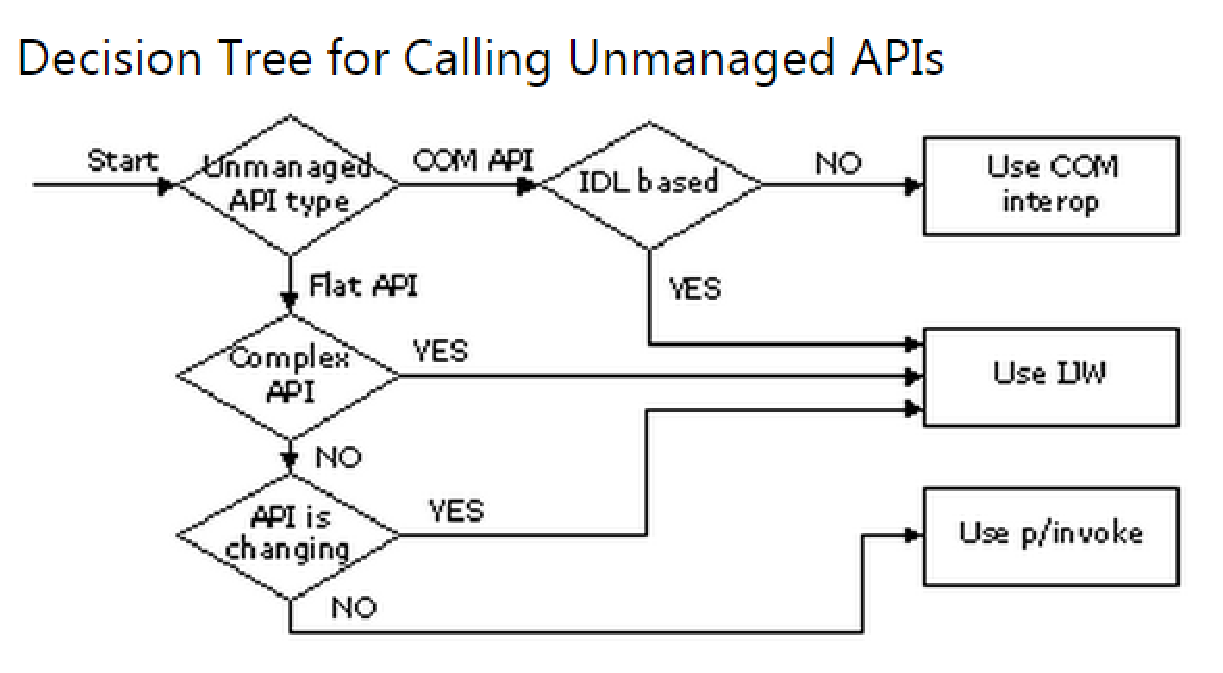
\includegraphics[height=6cm,
    angle=0]{./images/how2call_unmanagedAPI.eps}}
  \caption{Decesiion tree for calling unmanaged APIs}
  \label{fig:how2call_unmanagedAPI}
\end{figure}


Platform Invoke (P/Invoke) and COM (Component Object Model) interoperation
allows managed code to use native functionality.

P/Invoke provides the functionality to access functions, structs, and callbacks
in unmanaged DLLs. P/Invoke provides a translation layer to assist developers by
allowing them to extend the library of available functionality beyond the
managed library of the BCL. 

P/Invoke is a nice technology and it works fairly well, except for issues in
loading the target dll. We've found that the best way to do things is to create
a static library of native functions and link that into a Managed C++ (or
C++/CLI) project that depends upon it.  To call C++ code from C\#, one easy way
is to create a wrapper assembly in C++/CLI. In C++/CLI you can call into
unmanaged code as if you were writing native code, but you can call into C++/CLI
code from C\# as if it were written in C\#.

Example: Step 1 - C++/CLI
\begin{verbatim}
// compile: /CLR 
#include "NativeType.h"

public ref class ManagedType
{
     NativeType*   NativePtr; 

public:
     ManagedType() : NativePtr(new NativeType()) {}
     ~ManagedType() { delete NativePtr; }

     void ManagedMethod()
      { NativePtr->NativeMethod(); } 
}; 
\end{verbatim}

Example: Step 2 - in C\#
\begin{verbatim}
ManagedType mt = new ManagedType();
mt.ManagedMethod();
\end{verbatim}

Example: Step 1 - C++/CLI
\begin{verbatim}
#pragma managed(push, off)
#include "oldskool.h"
#pragma comment(lib, "oldskool.lib")
#pragma managed(pop)

using namespace System;

public ref class Wrapper {
private:
    COldSkool* pUnmanaged;
public:
    Wrapper() { pUnmanaged = new COldSkool; }
    ~Wrapper() { delete pUnmanaged; pUnmanaged = 0; }
    !Wrapper() { delete pUnmanaged; }
    void sampleMethod() { 
        if (!pUnmanaged) throw gcnew ObjectDisposedException("Wrapper");
        pUnmanaged->sampleMethod(); 
    }
};
\end{verbatim}

\subsection{Access COM APIs from managed code}


{\bf Suppose you have a COM and you want to use in .NET managed code}: 



There are only one way
\begin{enumerate}
  \item COM interop: available in all managed languages
\end{enumerate}
OLE Automation-compatible COM components. The CLR will take care of COM
component activation and parameter marshaling. 

COM interop relies on information from type libraries to make correct interop
calls, but type libraries typically do not contain all the information present
in IDL files. Using C++ interop solves this problem by allowing direct access to
these COM APIs.  

For companies that own COM APIs that have already shipped, it is important to
consider shipping primary interop assemblies (PIAs) for these APIs, thus making
them easy to consume for managed clients. 




\subsection{Access managed code from native code}


{\bf Suppose you have .NET managed code in assembly, and you want to use in C++ code}
\begin{itemize}
  \item write the C++/CLI code to mix the .NET managed code and C++ code (Sect.\ref{sec:C++/CLI}).
\end{itemize}


There are two main ways to expose a managed API to purely unmanaged callers
\begin{enumerate}
  \item as COM API via COM interop: enable call to COM APIs in any managed
  language from unmanaged code. COM interop is comprised of core services provided by the CLR,
  plus some tools and APIs in the System.Runtime.InteropServices namespace.
  
  Every public managed class can be exposed to unmanaged clients through COM
  interop. This process is easy to implement. Despite the fact that exposing
  managed APIs as COM APIs is easy, managed and COM object models are very
  different.
  Some features available in the managed world have no equivalent in the COM
  world and will not be usable from COM clients. Because of this, there is often
  tension between managed API design guidelines (DG) and compatibility with COM.
  
  Every managed class appears to implement IUnknown, IDispatch,
  ISupportErrorInfo, and a few other standard COM interfaces. 
  
  \item as a flat API (if the native code is C++)
  
  Sometimes unmanaged clients cannot use COM. For example, they might already be
  written to use flat APIs and cannot be changed or recompiled. C++ is the only
  high-level language that allows you to expose managed APIs as flat APIs. Doing
  this is not as straightforward as exposing a managed API as a COM API. It is a
  very advanced technique that requires advanced knowledge of C++ interop and
  the differences between the managed and unmanaged worlds.  
  
  \item (if the native code is C++ and we can recompile the C++ code into mixed
  mode image using VS.NET C++ compiler (i.e. C++/CLI compiler), then the
  unmanaged code can directly access any managed API) via C++ interop (sometimes referred to as It Just
  Works (IJW)) is a C++-specific feature, which enables flat APIs and COM APIs
  to be used directly, as they have always been used. This is more powerful than
  COM interop, but it requires much more care. Make sure that you check the C++
  resources before you use this technology.
  
  For C++ unmanaged clients that are willing to recompile their code with Visual
  Studio .NET, there is a third option: directly accessing managed
  functionality through C++ interop. Suggestions for how and when to use these
  options are described in this section.  
\end{enumerate}

C++/CLI programming language (See C/C++ manual book) let us write managed and
native code in the same program. First, compile the program with \verb!/clr!
switch, then the compiler create metadata for the application that can be
consumed by other managed asemblies, and enables the applications to consume
types and data in the metadata of other managed components.

\url{http://msdn.microsoft.com/en-us/library/ms717435(v=vs.100).aspx}


\subsection{Mixed code}

{\bf Suppose you want to write a program that accepts both native code and managed code}
\begin{itemize}	
  \item Managed C++ (Sect.\ref{sec:managed_C++}) 
  \item C++/CLI (Sect.\ref{sec:C++/CLI})
\end{itemize}


\section{.NET tools}
\label{sec:NET_tools}

.NET provde 3 new tools
\begin{enumerate}
  \item \verb!IntPtr!: a platform-dependent representation of a memory address
  \item \verb!GCHandle! :  can pin and retrieve the address of data in the
  managed memory heap
  \item \verb!Marshal! class: a one-stop portal for all memory operations, e.g.
  allocation, cleanup, and manipulaiton needs.
\end{enumerate}

In .NET 1.0 and 1.1, all operating system handles could be encapsulated only by
an \verb!IntPtr! object. However, this managed way to interact with unmanaged
resource is not safe.  IntPtr allowed handles to be leaked, particularly by
asynchronous exceptions. These exceptions present a huge hurdle for the garbage
collector (GC) being able to clean up those resources.  
To resolve such problems, .NET 2.0 then provides \verb!SafeHandle! and
\verb!ContrainedExecutionRegion! (CER) region. 
\url{http://www.codeproject.com/Articles/16157/SafeHandle-and-Constrained-Execution-Regions}



\section{IntPtr}
\label{sec:IntPtr}

\verb!IntPtr! is a structure to represent both addresses and handles (most
handles are pointers to Windows pointers). 
\begin{itemize}
  \item it is 32-bit on a 32-bit O/S
  \item it is 64-bit on a 64-bit O/S
\end{itemize}
Any function within the .NET Framework that exposes a way to work with addresses
and handles, uses the IntPtr type.

IMPORTANT: \verb!IntPtr! is similar to \verb!void *! in C/C++, i.e. a pointer
pointing to any object.

\section{SafeHandle vs. CriticalHandle vs. IntPtr}
\label{sec:SafeHandle}

\url{http://msdn.microsoft.com/en-us/library/ms182294.aspx}

\url{http://stackoverflow.com/questions/11973109/can-i-use-safehandle-instead-of-intptr}


\section{P/Invoke (.NET languages): Interop Marshalling}
\label{sec:marshalling}
\label{sec:P/Invoke}

.NET Framework 1.0 provides a way for managed code to call unmanaged functions
residing in DLLs, e.g. Win32 APIs.
P/Invoke: enable call any function in any unmanaged language as long as
  its signature is redeclared in managed source code. \textcolor{red}{If we just
  use a few flat APIs (or even complex flat APIs), then this is recommended to
  use.}
  
\begin{mdframed}
\textcolor{red}{complex flat API: APIs that have signatures that are hard to
declare in managed language. For example, methods with variable size structure parameters
are hard to declare since there is no equivalent concept in the managed type
system.}
\end{mdframed}
  
  
This include 3 primary steps in the managed
code
\begin{enumerate}
  \item declaration, i.e. define the interface of the unmanged code API (Sect.\ref{sec:P/Invoke_declaration}).
  
     At design time, we need to tell which unmanaged API you intend to call.
     This
includes (1) DLL name (i.e. the module), (2) function name (i.e. entry point),
(3) calling convention to use which includes Marshalling the data type so that
.NET understand the equivalent data type representation for parameter passing.
  
  \item invocation, i.e. calling the API via this interace
  
  
  \item error handling 
\end{enumerate}


\subsection{Declaration}
\label{sec:P/Invoke_declaration}

\subsubsection{Declaration: marshall functions}
\label{sec:marshall_API}

REQUIREMENT: The methods in the DLL need to be coded using 
\verb!__declspec(dllexport)! (Sect.\ref{sec:__declspec(dllexport)})
\begin{verbatim}
extern "C"  __declspec(dllexport) int MyMethod(int x)
{

}
\end{verbatim}

NOTE: We just provide the method declaration (ended with a semicolon) and it is
often use with \verb!DllImport! attribute.
\begin{itemize}
  \item we can put the API inside a class if we like
  

TIPS: It is suggested to put all APIs of a DLL inside the same class, within an
appropriate namespace. This class can be packaged in its own assembly and
distributed to all of the developers on your team or in your organization.
  
  \item alias can be used: the function name being used in the managed code can
  be different from the DLL's API. Then, \verb!EntryPoint! attribute need to be
  used to indicate the DLL's API name.
  
  
  \item another important thing is to use \verb!System.Runtime.InteropServices! in your
C\# code. The System.Runtime.InteropServices namespace provides a collection of
classes useful for accessing COM objects, and native APIs from .NET
  
  \item Final step, in order to build and run your C\# application, the DLL file must be
in the same folder of the C\# EXE file.
  
\end{itemize}
\begin{verbatim}
using System;
using System.Runtime.InteropServices;

class MyClass
{
  [DllImport("User32.dll")]
  public static extern Int32 MyMethod(Int32 x);
  
  
}

[DllImport("TestLib.dll")]

public static extern void DisplayHelloFromDLL ();

\end{verbatim}
The keyword \verb!extern! means that the method is implemented externally
(Sect.\ref{sec:keyword_extern}).


As \verb!Int32! is the equivalent .NET data type of C++ \verb!int! data type, there is no need for interop marshalling. The list of equivalent data type is given
\begin{verbatim}
C++ Type      .NET Framework Type           Blittable

bool           System.Boolean               N

signed char    System.SByte                 Y

unsigned char  System.Byte                  Y

wchar_t        System.Char                  N

double, long double
              System.Double                 Y

Float         System.Single                 Y

int, signed int, long, signed long
              System.Int32                  Y

unsigned int, unsigned long
              System.UInt32                 Y

__int64, signed __int64
             System.Int64                   Y

Unsigned __int64
             System.UInt64                  Y

short, signed short
             System.Int16                   Y

Unsigned short
             System.UInt16                 Y


\end{verbatim}
\url{http://www.codeproject.com/Articles/16987/C-Interop-is-for-the-Performance-Minded-Developer}

% In the C\# project, if we want to use the DLL above, in one source file, we add
% (suppose the DLL name is TestLib.dll, and the function we want to use from the
% DLL is DisplayHelloFromDLL())
% \begin{verbatim}
% \end{verbatim}

Example: define an alias
\begin{verbatim}
[DllImport("coredll.dll", EntryPoint="SHGetSpecialFolderPath")]
static extern bool GetFolderPath( //the rest of the declaration
\end{verbatim}
You can also define an alias of the function to use in managed code, and the
original name in unmanaged API should be given as the value of \verb!EntryPoint!
inside \verb!DllImport! attribute.


Example:
\begin{verbatim}
using System;
using System.Runtime.InteropServices;     // DLL support

class HelloWorld
{
    [DllImport("TestLib.dll")]
    public static extern void DisplayHelloFromDLL ();

    static void Main ()
    {
        Console.WriteLine ("This is C# program");
        DisplayHelloFromDLL ();
    }
}
\end{verbatim}

%\subsection{In the original DLL code}

Example:
\begin{verbatim}
[DllImport("coredll.dll", SetLastError=true)]
private static extern bool SHGetSpecialFolderPath(
   int hwndOwner, 
   string lpszPath,
   ceFolders nFolder,
   bool fCreate);
\end{verbatim} 
The function \verb!SHGetSpecialFolderPath! is marked as private as we only want
it to be called inside the class in which it is declared. Using \verb!extern!
modifier is required to indicate that the function is implemented externally
and using \verb!static! means the method can be called without creating an
instance of the class. The data type we use here must be the equivalent type
mentioned in Sect.\ref{sec:marshal_types}.
\url{http://msdn.microsoft.com/en-us/library/aa446536.aspx}

\begin{mdframed}
NOTE: coredll.dll is the Windows CE APIs equivalent to Win32 API filename: 
kernel32.dll, user32.dll.
\end{mdframed}




% \subsection{Expose function name inside a class}
% 
% At first, we need to wrap these unmanaged methods inside a class, i.e. declare
% the unmanaged function as a method of this class. To do so, we use \verb!DllImport! attribute which
% contains the DLL filename, then come the interface of the funciton using
% \verb!static extern! modifier.



\subsubsection{Declaration: marshall data types}
\label{sec:marshal_types}

During the invocation process (Sect.\ref{sec:invoke_wrapper-methods}), the
P/Invoke service is responsible for marshalling parameter values passed to the
DLL function. This is done by the component called {\bf marshaller} in the
P/Invoke service. 

There are two cases of data types: {\bf blittable types}
(Sect.\ref{sec:marshall_blittable-types}) and non-blittable data types.

\subsection{Passing blitable types}
\label{sec:marshall_blittable-types}

If the data type has the same representation between managed code and unmanaged
code, we call them {\bf blittable types} then the marshaller does not have to do
any special handdling to convert the data so that it is interpreted correctly by
the unmanaged code (i.e. marshalling process for the arguments) and
the managed code (i.e. unmarshalling process for the returned value). If the one
dimensional array of these blittable types, or even structure or classes that
contains only these types (except \verb!System.String!), the marshaller does not
have to do anything.

and we can use the right keyword
\begin{verbatim}
 System                     C# keyword-to-use        C/C++
System.Byte                   byte                   int
System.SByte                  sbyte
System.Int16                  short
System.UInt16                 ushort
System.Int32                  int
System.Int64                  long
System.UInt64                 ulong
System.IntPtr                 *   (using 'unsafe' keyword)


    (additional to .NET Compact Framework)
System.Char                    char
System.String                  string
System.Boolean                 bool
    
\end{verbatim}
As .NET Compact Framework only support Unicode, the  marshaler always marshals
System.Char as a 2-byte Unicode char and System.String as a Unicode
null-terminated array. Also, System.Boolean is marshalled as 1-byte integer
value; whereas .NET Framework use 4-byte integer value. 

At the time of invocation, \verb!System.String! is a reference type (it is
allocated in the managed heap, and the address is stored in the reference
variable), even though it is passed by value, the marshaller still passes a
pointer to the string to the unmanaged function.

IMPORTANT: .NET Compact Framework always passes a pointer to a reference type,
and does not support passing reference type by reference (i.e. using \verb!ref!
keyword in C\#), which makes the unmanaged code to see the string as one of the
following type
\begin{verbatim}
WCHAR*
TCHAR*
LPTSTR
LPSTR
\end{verbatim}
and manipulate the string using pointer (\textcolor{red}{This is different
from .NET Framework}). Nevertheless, when the function completes, the caller can
inspect the string as normal. 

In .NET Framework, the marshaler must take the character set into consideration.
As a result, the full .NET Framework does not support passing strings by value
or by reference into unmanaged functions and allowing the unmanaged function to
modify the contents of the buffer. Instead, we need to wrap the string into a
\verb!System.Text.StringBuilder! object and pass this object by pointer to the
unmanaged code. The only caveat is that if we decide to modify the content, the
object must be pre-allocated with enough space for the return value, or the text
will overflow, causing an exception thrown by P/Invoke service.

\begin{verbatim}
[DllImport("coredll.dll", SetLastError=true)]
private static extern bool SHGetSpecialFolderPath(
   int hwndOwner, 
   StringBuilder lpszPath,
   ceFolders nFolder,
   bool fCreate);


.............

Dim sPath As New StringBuilder(MAX_PATH)
ret = SHGetSpecialFolderPath(0, sPath, folder, False)
\end{verbatim}
 
IMPORTANT: Although System.String is a blittable type in the .NET Compact
Framework, it is not blittable when used inside a complex object, such as a
structure or class.

\subsection{Passing objects of structure or class type}

If the structure or class only contains data members of blittable types
(Sect.\ref{sec:marshall_blittable-types}), then you can pass directly the
structure or class type without worrying. The choose between struct and class is
that object of type struct is passed by value; while object of class type is
passed by reference. With pass by reference, marshaller always use a 4-byte
pointer to the reference type in the unmanaged code. Also, the layout of the
data members in the structure and the class is in the order in which they appear
in the managed code. However, to have a control on the layout, we can 
decorate the structure with \verb!StructLayout! attribute and
\verb!LayoutKind.Sequential! 

Example: when we define the wrapper method
\begin{verbatim}
// VB.NET
Private Structure MEMORY_STATUS
  Public dwLength As UInt32
  Public dwMemoryLoad As UInt32
  Public dwTotalPhys As UInt32
  Public dwAvailPhys As Integer
  Public dwTotalPageFile As UInt32
  Public dwAvailPageFile As UInt32
  Public dwTotalVirtual As UInt32
  Public dwAvailVirtual As UInt32
End Structure

<DllImport("coredll.dll", SetLastError:=True)> _
Private Shared Sub GlobalMemoryStatus(ByRef ms As MEMORY_STATUS)
End Sub
\end{verbatim}

\begin{mdframed}
In .NET Compact Framework, the marshaller cannot marshall complex objects
(reference types) within structures. This means that if the structure contain a
member of a type not of blittable types, the structure cannot be fully
marshalled. 
\end{mdframed}

To marshall a complex object in .NET Framework, we use \verb!MarshallAs!
attribute, to explicitly tell the marshaller how to marshall the data members. 

\subsection{Invoke the wrapped method}
\label{sec:invoke_wrapper-methods}

After you define the class with the methods marshalling the unmanaged APIs
(Sect.\ref{sec:marshall_API}) and the equivalent data types
(Sect.\ref{sec:marshal_types}), we can compile the class into an assembly, and
use it as a regular managed code inside another managed code.

As the wrapper method can raises an error, whenever we call it, we need to wrap
inside a \verb!try/catch! block (Sect.\ref{sec:marshall_handling-errors}
describes potential exceptions)
\begin{verbatim}

public string MyFunctionUseUnmanagedFunction()
{ 
   try{
     ret = SHGetSpecialFolderPath(0, sPath, folder, False);
   }
   catch (ex As Exception)
   {
        HandleCeError(ex, "GetSpecialFolderPath");
        Return Nothing;
   }   
   if (!ret)
   {
    // API error and retrieve error number
    int errNum = Marshal.GetLastWin32Error();
   }
   
   return sPath;
}      
\end{verbatim}

At runtime, the code is JIT compiled at runtime and the P/Invoke service of the
CLR extracts the \verb!DllImport! definition from the metadata of the assembly,
locate and load the DLL containing the function into memory, and then retrieve
the address of the function using the entry point information.
If all goes well, the function will then be invoked, its arguments marshaled,
and any return values passed back to the caller.

\subsection{Handling errors}
\label{sec:marshall_handling-errors}


Although developers never expect their code to generate runtime errors, it is
important to remember that functions invoked on DLLs using P/Invoke can generate
two different kinds of errors.
\begin{enumerate}
  \item \verb!NotSupportedException! is raised: exception generated by the
  P/Invoke service itself, i.e. when the arguments passed to the method
  contains invalid data, or the function is declared with incompatible interface with the entrypoint's function in
  unmanaged DLL.
  
  \item \verb!MissingMethodException! is raised: P/Invoke service throw this
  exception if the entrypoint is not found in the unmanaged DLL.
\end{enumerate}


\subsection{TIPS: string encoding}


\section{Using pointers: unsafe code}

In CLR,  unsafe code is referred to as unverifiable code.Unsafe code in C\# is
not necessarily dangerous; it is simply code whose safety cannot be verified by
the CLR. Also, remember that  unsafe code cannot be executed in an untrusted environment.
For example, you cannot run unsafe code directly from the Internet.


Using pointers in C\# is recommended in scenarios
\begin{enumerate}
  \item performance-critical code
  
Example: In situations where you are doing extremely intensive operations
against large blobs in memory, for example image manipulation, it is faster to
step outside the normal safety the runtime provides.


  \item advanced COM or P/Invoke scenarios that involves structures with pointer
  in them.
  \item dealing with existing structures on disk
\end{enumerate}

There, we need to put the code inside \verb!unsafe! context to allow pointers.

\section{C++ interop (Visual C++): dllexport, dllimport}
\label{sec:interop_C_Csharp}

Since Visual Studio 2005, Visual C++ (under the name C++/CLI -
Sect.\ref{sec:C++/CLI} of C/C++ manual book) supports interoparability that
enables both managed code and unmanaged code to exist in the same application,
and even in the same file (using \verb!#managed!, \verb!#unmanaged! pragmas).
Visual C++ supports the creation of three distinct types of components and
applications: mixed, pure, and verifiable. All three are available through the
\verb!/clr! (Common Language Runtime Compilation) compiler option.

C++ interop (available in C++): it requires to introduce a whole new
  module written in C++. So use this if the unmanaged flat APIs are changing
  while managed code is under development. The C++ layer can be very thin and
  the rest of the managed code can be written in any other managed language of
  choice. Using C++ interop solves this problem by allowing direct access to
  unmanaged APIs - which requires no rewriting, just the inclusion of a header
  file. 

This allows Visual C++ to integrate .NET functionality into existing Visual C++
applications without disturbing the rest of application. 

C++ Interop is better than P/Invoke (Sect.\ref{sec:P/Invoke}) if the interface
of the functions from DLL keeps changing. It also provides better type safety,
and make performance enhancements possible that are not possible with P/Invoke.
C++ Interop uses the fastest possible method of data marshaling, whereas
P/Invoke uses the most robust method. This means that C++ Interop (in a fashion
typical for C++) provides optimal performance by default, and the programmer is
responsible for addressing cases where this behavior is not safe or appropriate.  
 
However, C++ Interop is not possible if the unmanaged source code is not
available or when compiling with /clr:safe

% \section{C++ COM Interop}
% 

% 
% 
% \section{C++ code call managed classes directly}
% 
% 
% There are two options
% \begin{enumerate}
%   \item make the C++ code become C++/CLI code, by compiling with \verb!/clr! options
%   
%   \item wrap the managed classes in a DLL with native entry points
% \end{enumerate}

\section{/clr option}
\label{sec:clr_option}

The \verb!/clr! option is used to compile mixed code (managed + native) -
Sect.\ref{sec:managed_C++} and Sect.\ref{sec:C++/CLI}.
There are different options, Fig.\ref{fig:clr_option}.
\url{https://msdn.microsoft.com/en-us/library/k8d11d4s.aspx}

\begin{figure}[hbt]
  \centerline{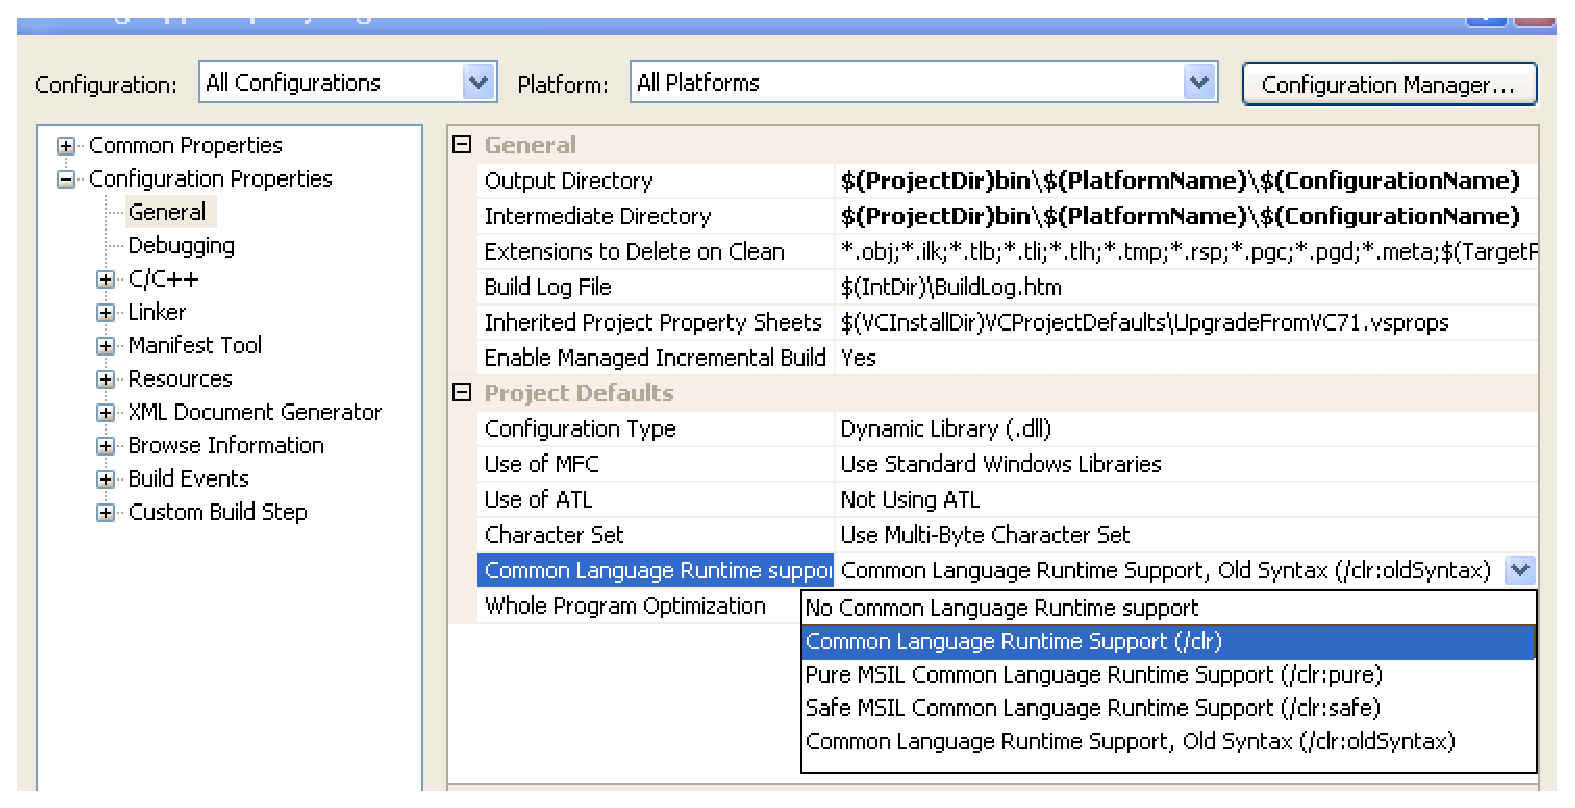
\includegraphics[height=2.7cm,
    angle=0]{./images/clr_option.eps}}
\caption{/clr options}
\label{fig:clr_option}
\end{figure}


\begin{verbatim}
Project properties
   Configuration Properties
      General
\end{verbatim}
There are a few options:
\begin{enumerate}
  \item No Common Language Runtime Support: compile your code as native code

  \item Common Language Runtime Support, Old syntax (/clr:oldSyntax) : compile Managed C++ code (Sect.\ref{sec:managed_C++}) in Visual Studio 2008 and above. 
  
  This can be removed anytime in the future.
  
  \item Common Language Runtime Support (/clr): compile C++/CLI code
  
  \item Pure MSIL Common Language Runtime Support (/clr:pure): Produces a Microsoft Intermediate Language (MSIL)-only output file that has no native executable code. However, it can contain native types compiled to MSIL. 
  
  \item Safe MSIL Common Language Runtime Support (/clr:pure): Produces an MSIL-only (no native executable code)
  
\end{enumerate}

\url{http://stackoverflow.com/questions/4094832/converting-from-c-cli-oldsyntax-how-to-and-can-this-be-automated}

The mixed code can be an executable file, or a library. 
\begin{itemize}
  \item To enable debugging: add \verb!/ASSEMBLYDEBUG! 
  \url{https://msdn.microsoft.com/en-us/library/cta4x5hc.aspx}
  
  \item Use \verb!#pragma unmanaged! to specify the region of code to be compiled to native code.
  and use \verb!#pragma managed! to switch back to managed code region.
   
  \item Code must be compiled with \verb!/MD!, which ensure 
  the dynamically linked, multithreaded versions of the runtime routines are selected from the standard header. 
  This is a known limitation as the CLR garbage collector runs finalizers on a different thread.
   
\end{itemize}
\url{https://msdn.microsoft.com/en-us/library/k8d11d4s.aspx}

\section{Troubleshoot}


In VS 2008 (Sect.\ref{sec:VS_2008}),  the 32-bit mixed code can give an
exception about some code that was not created on the managed heap, when
something calls \verb!CrtIsValidHeapPointer()!. A solution was
adding 
\begin{verbatim}
__DllMainCRTStartup@12
\end{verbatim}
to 
\begin{verbatim}
Project properties
   Linker 
     Input
        Force Symbol References
         __DllMainCRTStartup%4012;%(ForceSymbolReferences)
\end{verbatim}

However, in 64-bit application, this gives an error
\begin{verbatim}
Linking...
1>LINK : error LNK2001: unresolved external symbol __DllMainCRTStartup@12
-------------------
\end{verbatim}
A solution for 64-bit application is adding
\begin{verbatim}
_DllMainCRTStartup

// or

_DllMainCRTStartup;%(ForceSymbolReferences) 
\end{verbatim}
(one underscore, no "@12" postfix) as the exported functions are not decorated
\url{https://social.msdn.microsoft.com/Forums/en-US/bf162181-864c-4c25-88b0-b56d1affe350/crtisvalidheappointer-vs-dllmaincrtstartup12-in-vs2008-x64?forum=netfx64bit}